\documentclass[11pt]{article}

\usepackage[T1]{fontenc}
\usepackage[utf8]{inputenc}
\usepackage{lmodern}
\usepackage[margin=1in]{geometry}
\usepackage{microtype}
% Keep command-line double hyphens literal in typewriter text.
\DisableLigatures[-]{encoding = T1, family = tt*}
\usepackage{amsmath}
\usepackage{booktabs}
\usepackage{longtable}
\usepackage{tabularx}
\usepackage{array}
\newcolumntype{L}[1]{>{\raggedright\arraybackslash}p{#1}}
\usepackage{xcolor}
\usepackage{enumitem}
\usepackage{listings}
\usepackage{fancyhdr}
\usepackage{tikz}
\usetikzlibrary{arrows.meta,calc,fit,positioning}
\usepackage[hidelinks]{hyperref}

% Keep the generated PDF stable across identical builds with pdfTeX.
\pdfinfoomitdate=1
\pdftrailerid{}
\pdfsuppressptexinfo=15

\definecolor{pipelineblue}{HTML}{315E7D}
\definecolor{lightblue}{HTML}{EDF4F8}
\definecolor{lightgold}{HTML}{FFF7E6}
\definecolor{lightgreen}{HTML}{EAF5EF}
\definecolor{lightpurple}{HTML}{F2ECF8}
\definecolor{codegray}{HTML}{F4F5F6}

\hypersetup{
  pdftitle={Drosophila cCRE pipeline: detailed implementation},
  pdfauthor={drosophila-cCREs project},
  pdfsubject={ATAC-seq and H3K27ac processing, master DHS registry, context-resolved regulatory catalog, and nearest-TSS annotation for an eight-context dm6 atlas}
}

\pagestyle{fancy}
\fancyhf{}
\fancyhead[L]{Drosophila cCRE pipeline}
\fancyhead[R]{Detailed implementation}
\fancyfoot[C]{\thepage}
\setlength{\headheight}{14pt}

\setlist[itemize]{leftmargin=1.6em,itemsep=0.25em,topsep=0.35em}
\setlist[enumerate]{leftmargin=1.8em,itemsep=0.3em,topsep=0.35em}
\setlength{\parindent}{0pt}
\setlength{\parskip}{0.55em}
\setlength{\emergencystretch}{3em}
\renewcommand{\arraystretch}{1.18}

\lstdefinestyle{pipelinecode}{
  basicstyle=\ttfamily\small,
  backgroundcolor=\color{codegray},
  frame=single,
  rulecolor=\color{gray!35},
  breaklines=true,
  columns=fullflexible,
  keepspaces=true,
  showstringspaces=false,
  xleftmargin=0.3em,
  xrightmargin=0.3em
}
\lstset{style=pipelinecode}

\newcommand{\stage}[1]{\texttt{#1}}
\newcommand{\filep}[1]{\path{#1}}
\newcommand{\software}[1]{\textsf{#1}}

\title{\textbf{Drosophila cCRE Pipeline}\\[0.3em]
\large Detailed implementation and scientific reasoning}
\author{drosophila-cCREs project}
\date{Repository documentation revision: 2026-10-10}

\begin{document}

\maketitle

\begin{abstract}
This document describes the implemented workflow that converts public ATAC-seq
and IP-only H3K27ac accessions into quality-reviewed biological-library BAMs,
replicate-supported context peaks, a variable-width summit-aware master
DNase-hypersensitive-site (DHS) registry, and a context-resolved catalog of
candidate \emph{cis}-regulatory elements.  The published dm6 atlas covers eight
contexts built from 20 ATAC-seq and 14 H3K27ac biological libraries.  The
catalog combines ATAC accessibility with H3K27ac signal using assay-specific
background TMM normalization, the maximum of three 500-bp summit windows, and a
context-specific empirical background of nonmember DHSs; a member DHS is called
active when its background percentile exceeds a configurable threshold
(default 0.60).  Every enhancer-like element is then assigned to its nearest
annotated TSS, with exact ties kept in one row and promoter activity annotated
in every context.  Portable browser tracks, IGV sessions, and an integrated
checksummed report accompany the tables.  Each section states what the rules
do, why that choice was made, and which limitations remain.  This is
implementation documentation for the live \filep{workflow/Snakefile} and its
rule files; it does not replace inspection of the resolved configuration and
provenance of a particular run.
\end{abstract}

\tableofcontents
\newpage

\section{Purpose and scope}

The pipeline has three related scientific goals:

\begin{enumerate}
  \item construct a stable atlas coordinate system---the master DHS
  registry---from reproducible ATAC accessibility evidence across the contexts
  named in the input table;
  \item annotate every master DHS in every context with accessibility,
  H3K27ac max3 background percentile, an activity call, TSS proximity, and
  blacklist overlap; and
  \item assign every enhancer-like element to its nearest annotated TSS and
  annotate that promoter's activity across contexts, without turning proximity
  into a causal target assignment.
\end{enumerate}

The published atlas is defined entirely by two versioned tables.
\filep{resources/atlas_samples.tsv} lists 35 public accessions forming 34
biological libraries: 20 ATAC-seq and 14 IP-only H3K27ac libraries across the
eight contexts \texttt{ab}, \texttt{e13}, \texttt{e5}, \texttt{ead},
\texttt{hid}, \texttt{lb}, \texttt{o}, and \texttt{wid}.
\filep{resources/atlas_qc_decisions.tsv} records one QC decision per library
and the reviewed fragment length of every single-end H3K27ac library.

The public interface is accession-first.  Users provide public accessions and
biological metadata, not raw FASTQ paths.  The canonical launcher is
\filep{src/run_pipeline.py}; it validates inputs, resolves defaults and
accession layouts, writes a deterministic YAML configuration, and invokes the
canonical \filep{workflow/Snakefile}.  Snakemake then owns dependency tracking,
resource scheduling, rule environments, and restart behavior.

The workflow comprises ATAC-seq and H3K27ac processing, H3K27ac-based context
activity annotation, catalog visualization, nearest-TSS candidate-gene
annotation, and integrated reporting.  It does not import an external
regulatory-element catalog or apply quantile normalization.  The continuous
signals and frozen master coordinates are exported so that further
enhancer--gene analyses can be performed downstream.

\section{The data model}

\subsection{Run, library, context, and assay}

Four identifiers have distinct meanings:

\begin{description}[style=nextline,leftmargin=2.2em]
  \item[Accession or technical run]
  One public run, or one run obtained by expanding a public experiment
  accession.  Technical runs are processed independently through trimming and
  alignment.

  \item[Biological library]
  The unit identified by \texttt{library\_id}.  Multiple technical runs may
  share one library ID.  Their aligned BAMs are merged before duplicate
  marking so duplicates are defined across the complete biological library.

  \item[Context]
  The tissue or developmental stage in the sample-sheet \texttt{context}
  column.  Distinct ATAC libraries in one context are biological replicates.
  The same context label links accepted ATAC and H3K27ac libraries during
  activity quantification.

  \item[Assay]
  Either \texttt{atac} or \texttt{h3k27ac}.  H3K27ac rows are processed by the
  histone ChIP branch (internal assay namespace \texttt{chip\_histone}) and
  retained as H3K27ac in the downstream atlas.
\end{description}

Collapsing these levels would create pseudoreplication or biased weights.  A
technical lane is not a biological replicate; a library should receive one
QC decision; and a context estimate should give equal weight to accepted
biological libraries rather than to the number of sequencing lanes.

\subsection{Canonical sample sheet}

The CSV or TSV input conforms to
\filep{schemas/sample-sheet.schema.yaml}.  Four columns are required:

\begin{center}
\begin{tabularx}{0.94\textwidth}{>{\ttfamily}l X}
\toprule
\normalfont Column & Meaning \\
\midrule
accession & Public run or experiment accession (SRR/SRX/ERR/ERX); experiments expand to their runs. \\
library\_id & Biological library identifier; shared by technical runs only. \\
assay & \texttt{atac} or \texttt{h3k27ac}; selects the processing branch and its defaults. \\
context & Replicate-pooling and downstream atlas group. \\
\bottomrule
\end{tabularx}
\end{center}

Optional per-row fields override adapters, trimming, alignment, filtering, and
MACS3 parameters; the atlas uses the defaults throughout.  Rows sharing a
library ID must agree on context, assay, and every processing field.  H3K27ac
libraries are IP-only: input-control columns are rejected, and MACS3 estimates
its local lambda from the IP library.  Each ATAC context needs at least two
biological libraries.

The genome is the project-level launcher argument \texttt{--genome dm6}, and
sequencing layout is resolved from accession metadata.  Per-row genome or raw
FASTQ fields are deliberately absent from the public contract.

\section{Staged execution and the manual checkpoint}

\subsection{Why there are separate invocations}

The workflow is intentionally not one uninterrupted accession-to-catalog job.
It is organized around immutable, checksummed artifacts and an explicit
library-review boundary:

\begin{center}
\fcolorbox{pipelineblue}{lightblue}{%
\begin{minipage}{0.92\textwidth}
\textbf{Invocation 1: accessions $\rightarrow$ QC}\\
download $\rightarrow$ trim $\rightarrow$ align $\rightarrow$ peaks and QC
$\rightarrow$ pending final-BAM manifests and library review table

\vspace{0.35em}
\centering $\Downarrow$ \quad \textbf{recorded pass/fail decisions} \quad $\Downarrow$

\raggedright\vspace{0.35em}
\textbf{Invocation 2: reviewed ATAC BAMs $\rightarrow$ master}\\
validate $\rightarrow$ accepted ATAC replicate/context peaks $\rightarrow$
master DHS bundle

\vspace{0.35em}
\textbf{Invocation 3: reviewed BAMs + frozen master $\rightarrow$ catalog/links/report}\\
validate $\rightarrow$ count $\rightarrow$ normalize $\rightarrow$ annotate
$\rightarrow$ nearest-TSS links $\rightarrow$ tracks, IGV sessions, and report
\end{minipage}}
\end{center}

There is no interactive pause inside Snakemake.  Decisions are applied to each
per-assay final-BAM manifest with \filep{src/review_final_bam_manifest.py},
which writes a new reviewed manifest and never edits the generated one.  For
the published atlas the decisions are the versioned
\filep{resources/atlas_qc_decisions.tsv}, and \texttt{--assay atac} or
\texttt{--assay h3k27ac} selects the rows belonging to each manifest.  For a new
dataset, the generated \filep{qc/library-review.tsv} is copied outside the
result namespace and completed.  The tool requires exactly one decision per
manifest library and a reason for every failure.  A master run rejects any
pending ATAC decision, and quantification requires reviewed ATAC and H3K27ac
manifests.

An automatic pipeline can calculate metrics but cannot decide whether a
library is biologically fit for a specific atlas.  Making the review boundary
an explicit file transformation preserves that judgment without hiding it in
an interactive process or modifying generated manifests in place.

\subsection{Input and stopping stages}

\begin{longtable}{>{\ttfamily}p{0.18\textwidth} L{0.34\textwidth} L{0.35\textwidth}}
\toprule
\normalfont Start & Required starting artifact & Allowed endpoints \\
\midrule
\endhead
accessions & Sample sheet plus resolved, checksummed download manifest &
\stage{trimming}, \stage{alignment}, or \stage{qc} \\
trimming & Checksummed trimming checkpoint &
\stage{trimming}, \stage{alignment}, or \stage{qc} in the source namespace \\
alignment & Checksummed alignment checkpoint or complete final-BAM manifest &
\stage{alignment} or \stage{qc} \\
qc & QC checkpoint plus a reviewed ATAC final-BAM manifest for master construction &
\stage{qc} or \stage{master} \\
master & Checksummed master bundle and reviewed ATAC/H3K27ac BAM manifests when continuing &
\stage{master}, \stage{quantification}, \stage{catalog}, \stage{links}, or \stage{report} \\
quantification & Checksummed quantification checkpoint &
\stage{quantification}, \stage{catalog}, \stage{links}, or \stage{report} \\
catalog & Checksummed catalog checkpoint, or an immutable catalog-bundle manifest &
\stage{catalog}, \stage{links}, or \stage{report} from a checkpoint; \stage{links} only from a bundle manifest \\
links & Checksummed nearest-TSS link checkpoint & \stage{links} or \stage{report} \\
report & Checksummed report checkpoint & \stage{report} validation \\
\bottomrule
\end{longtable}

Each endpoint exports
\filep{provenance/manifests/<stage>.checkpoint.json}.  It records the stage,
scientific semantic digest, complete peak/refinement parameters where relevant,
and SHA-256 hashes of the restart artifacts.  Its stage-specific resolved
configuration snapshot is retained below \filep{provenance/configs/}, so
advancing the same run does not invalidate an earlier boundary.  Advancing
\texttt{--until-stage} inside an allowed start mode changes only requested
targets; it is excluded from the scientific semantic digest.

Strict reuse modes have no upstream fallback.  For example, a quantification
run cannot silently redownload or realign a missing library.  It first verifies
the declared files, SHA-256 hashes, genome, BAM/index coherence, coordinate
compatibility, and filtering contract.

\section{Reference preparation}

dm6 reference construction belongs to the workflow DAG.  The resolved
configuration records the UCSC dm6 FASTA, the UCSC-distributed NCBI RefSeq GTF
(\filep{dm6.ncbiRefSeq.gtf.gz}), and the Boyle-lab Blacklist v2 dm6 BED,
together with their checksums.  The workflow:

\begin{enumerate}
  \item downloads archives with resumable \software{aria2} transfers and
  integrity checking;
  \item decompresses the FASTA and blacklist through temporary files followed
  by atomic replacement;
  \item builds the \software{samtools faidx} and \software{Bowtie2} indexes;
  \item derives chromosome sizes in FASTA order;
  \item extracts one-base TSS records from the annotation; and
  \item writes the configured autosome list used for background normalization.
\end{enumerate}

The blacklist is an annotation reference rather than an alignment filter.  At
the catalog stage, master-DHS overlap with it is reported as a binary flag, an
overlapping-base count, and a fraction of the master interval, and it defines
which DHSs may enter the H3K27ac activity background.  The TSS BED supports
ATAC TSS enrichment and regulatory-class annotation.  The autosome list
excludes sex chromosomes and mitochondrial DNA from the TMM background matrix.

Reference identity is part of the computation, not a machine-local
prerequisite.  Checksummed preparation in the DAG makes alignment, QC,
normalization, and coordinates traceable to the same assembly and avoids
silent reuse of a similarly named but different reference.

\section{Acquisition, read QC, and trimming}

\subsection{Checksummed acquisition}

Run and experiment accessions are normalized and experiments are expanded to
their constituent runs.  Acquisition produces immutable compressed FASTQs and
a manifest with resolved paths, layout, and checksums.  After \software{aria2}
validates an ENA MD5, the downloader atomically writes a small
\texttt{.verified.json} sidecar containing the expected checksum, expected and
observed sizes, and file modification metadata.  A restart skips the expensive
rehash only when that record still matches both the newly resolved ENA
metadata and the current file; a missing or stale record sends the FASTQ back
through \software{aria2} integrity validation.  Successfully validated files
receive their records even when another URL in the same batch fails.
In the default \texttt{--backend auto} mode, runs whose direct ENA FASTQs fail
transfer or integrity validation are converted with SRA Toolkit; ENA files
from other runs that completed successfully remain in place.  SRA-derived
files are promoted only after conversion and compression complete.  Explicit
\texttt{--backend ena} mode disables this failover.  The
\texttt{--skip-download} path reuses an existing manifest after validation.

\subsection{Raw and trimmed read assessment}

Every technical run and mate receives raw \software{FastQC}.  Reads are then
trimmed with \software{Cutadapt}; defaults are Nextera adapters for ATAC and
TruSeq adapters for H3K27ac, quality cutoff 20, minimum retained length 20 bp,
error rate 0.1, and minimum adapter overlap 3 bp.  Paired-end trimming is
synchronized.  FastQC is repeated on the trimmed output, and Cutadapt writes a
JSON record used by MultiQC.

Running QC before and after trimming separates properties of the deposited
reads from effects introduced by processing.  Keeping technical runs separate
at this stage reveals lane-specific failures before they are hidden by a
library merge.

\section{Alignment and biological-library BAM construction}

\subsection{Lane alignment}

Each trimmed technical run is aligned independently with \software{Bowtie2}.
The default preset is \texttt{--very-sensitive}.  For paired-end data, the
workflow also uses \texttt{--no-mixed}, \texttt{--no-discordant}, and a default
maximum fragment length of 2,000 bp.  Read-group IDs identify the technical
run while the sample field identifies the biological library.

The streamed alignment is converted to BAM, name-sorted, processed with
\software{samtools fixmate -m}, and coordinate-sorted.  Temporary intermediates
are checked with \software{samtools quickcheck}.  With
\texttt{--alignment-chunk-pairs} \(n\), very large lanes are split into chunks
of \(n\) read pairs (or reads for single-end data), each chunk is aligned as an
independent restartable job, and the coordinate-sorted chunks are merged back
into one lane BAM with aggregated Bowtie2 statistics.  Chunking changes only
scheduling and restart granularity, not the alignment parameters.

\subsection{Merge, duplicate marking, and filtering}

All lane BAMs sharing a biological library ID are merged.  Duplicate marking
is then performed once over the merged library.  The final filter applies:

\begin{itemize}
  \item minimum MAPQ 30 by default;
  \item exclusion of unmapped, secondary, QC-failed, and supplementary
  alignments;
  \item proper-pair and mapped-mate requirements for paired-end libraries;
  \item duplicate exclusion when \texttt{remove\_duplicates=true};
  \item mitochondrial-contig removal by default.
\end{itemize}

Blacklist-overlapping alignments are deliberately retained so that the same
unfiltered signal supports peak calling and quantitative annotation.  The
resulting elements are then flagged by their recorded overlap rather than
disappearing before inspection.

The result is a coordinate-sorted final BAM and BAI.  Flagstat, stats, and
idxstats summaries are calculated for every biological library.  At the
\stage{alignment} boundary the workflow exports a checksummed final-BAM
manifest; newly generated rows have \texttt{qc\_status=pending\_review}.
Every row carries the filtering contract
\texttt{short-read-processing-final-v2}, which records this
blacklist-retaining behavior.  Master-bundle manifests record the input
filtering contract as well, and every downstream reuse requires it to match.

Duplicate marking before technical-run merging would miss molecules duplicated
across lanes.  Conversely, merging biological replicates would erase the
replicate structure required for reproducibility checks.  The chosen order
therefore matches the experimental unit.

\section{Peak calling}

\subsection{Paired-end ATAC: Tn5/MACS3-qpois}

The ATAC implementation is explicitly insertion-based:

\begin{enumerate}
  \item Retain proper pairs with nonzero template length and
  \(0 < |\mathrm{TLEN}| < 150\) bp by default.  Unmapped, mate-unmapped,
  secondary, QC-failed, duplicate, and supplementary records are excluded.
  \item Apply the Tn5 offset with \software{alignmentSieve --ATACshift}.
  \item Convert both shifted mates to separate one-base insertion records.  A
  consistency check requires the shifted alignment count to equal the number
  of insertion records.
  \item Run \software{MACS3 callpeak} on the BED input with
  \texttt{-f BED --nomodel --shift -75 --extsize 150 --keep-dup all -B
  -q 0.10}.  The pileup and local lambda are deliberately unscaled; this
  branch must not use \texttt{--SPMR}.
  \item Clip the treatment pileup and local lambda to chromosome bounds and
  calculate the qpois signal with \software{macs3 bdgcmp -m qpois}.
  \item Refine candidate peaks over qpois exponents 2 through 325.  Connected
  components shorter than 50 bp are rejected; components at most 400 bp are
  retained; wider components are followed to higher exponents so that they can
  split into narrower subcomponents.  The default merge gap is one base.
\end{enumerate}

This sequence runs for each accepted biological replicate and again on pooled
insertions within each context.  The pooled call provides context boundaries
and signal; the replicate calls provide reproducibility evidence.
The QC endpoint freezes each refined replicate BED together with the complete
MACS3 and qpois-refinement parameter mappings.  A QC-to-master invocation
validates and reuses those lenient replicate calls, while still constructing
the pooled context calls.  It refuses reuse if the requested q-value, Tn5
geometry, exponent range, component lengths, or merge gap differs.

Two-ended Tn5 insertions represent cut sites more directly than treating an
ATAC fragment as a ChIP enrichment interval.  Computing qpois from unscaled
pileup and lambda preserves MACS3's intended count-scale comparison.
Progressive refinement constrains the geometry of broad candidates, but it is
not an additional independent FDR-controlled test; candidate q-values remain
the statistical starting point.

\subsection{H3K27ac QC peaks}

Each H3K27ac library is called by the rule \texttt{callpeak\_h3k27ac} with
\texttt{macs3 callpeak --broad --broad-cutoff 0.1 -q 0.01 -B --SPMR} and no
\texttt{-c} argument, so MACS3 estimates the local lambda from the IP library
itself.  The MACS3 input format resolves from the library layout.  Outputs are
the broadPeak and gappedPeak files, the MACS3 table, and SPMR-scaled
treatment-pileup and local-lambda bedGraphs.  The SPMR behavior is
intentionally different from the ATAC qpois branch.

These peaks are QC evidence only: they supply the H3K27ac peak count and FRiP
used during library review.  The catalog never consumes H3K27ac peak calls;
it quantifies H3K27ac directly from BAM-derived fragment units around master
DHS summits (Sections~\ref{sec:quantification}--\ref{sec:activity}).  Calls
without an input control are adequate for this purpose, but they should not be
interpreted as a control-normalized enrichment test.

\section{Quality control and library review}

The QC endpoint combines general and assay-specific evidence:

\begin{itemize}
  \item raw/trimmed FastQC and Cutadapt metrics;
  \item final-BAM flagstat, stats, and idxstats;
  \item peak count and fraction of reads in peaks (FRiP);
  \item ATAC TSS profiles over \(\pm2\) kb, derived from temporary Tn5-shifted
  CPM tracks, and fragment-length histograms;
  \item \software{phantompeakqualtools} cross-correlation, fragment-shift
  estimates, NSC, RSC, and quality tags for H3K27ac libraries; and
  \item a MultiQC report and one consolidated review row per library.
\end{itemize}

For paired-end libraries, FRiP uses one valid same-chromosome fragment per read
pair in the denominator and counts a fragment once if it overlaps any called
peak.  For single-end libraries, the unit is one filtered read.  Thus FRiP is
fragment-aware and is not inflated by counting two mates independently.

ATAC TSS enrichment is calculated from the aggregate 4-kb profile as the
maximum signal in the central \(\pm50\)-bp interval divided by the mean signal
in the two terminal 100-bp flanks.  The review table also reports the median
ATAC fragment length, fraction below 150 bp, and fraction from 180--250 bp.

The reviewer edits only \texttt{qc\_decision} (\texttt{pass} or
\texttt{fail}), \texttt{estimated\_fragment\_length\_bp}, and \texttt{notes}.
A failed row requires a reason.  Single-end H3K27ac also requires a reviewed
positive fragment length; the cross-correlation estimate is pre-populated as a
suggestion rather than accepted silently, and the field must stay blank for
every other library.  In the published atlas all 34 libraries pass, and the
seven single-end H3K27ac libraries carry reviewed fragment lengths.

No universal numeric cutoff is safe across all public datasets.  The table
puts depth, mapping, enrichment, fragment structure, and visual evidence next
to the decision so inclusion criteria can be documented at library resolution.

\section{Context peak reproducibility}

Accepted ATAC libraries are grouped by the sample-sheet context.  Their
insertion BEDs are concatenated and a pooled qpois context call is made and
refined.  The pooled peaks are not accepted merely because they are present in
the aggregate signal.

For every pooled peak \(P\), each replicate peak set is reduced to an interval
union and the coverage fraction is calculated:

\[
  f_r(P) = \frac{|P \cap U_r|}{|P|},
\]

where \(U_r\) is the union of replicate \(r\)'s peaks.  A replicate supports
the pooled peak when \(f_r(P) \geq 0.5\) by default.  The peak is retained when
at least two biological libraries support it.  Both thresholds are launcher
parameters, and the minimum cannot exceed the accepted replicate count.  The
support table retains every pooled peak, all per-replicate fractions, the
supporting library list, and the retain/reject decision.

Pooled data improve sensitivity and define a context-level signal, but pooling
alone can promote a feature driven by one library.  Requiring substantial
coverage in multiple independent biological libraries makes reproducibility
an explicit property of every retained context peak.

\section{Summit-aware master DHS registry}

The master registry is built only from replicate-supported context peaks.  It
is neither a simple interval union nor a fixed-width resizing operation.

\subsection{Context summits}

For each source peak, the workflow reads the pooled context BigWig and chooses
the maximum-signal base.  If the maximum occupies more than one plateau, it
selects the midpoint of the plateau closest to the peak midpoint, with a
leftmost deterministic tie break.  If no finite signal is available, it uses
the peak midpoint and records a summit fallback.

\subsection{Cross-context clustering}

Source peaks are processed by chromosome.  A peak can join a cluster only if:

\begin{itemize}
  \item its context is not already represented in that cluster;
  \item the complete span of member summits remains at most 150 bp by default;
  and
  \item it reciprocally contains a summit with at least one current member:
  each of the two peak intervals contains the other's summit.
\end{itemize}

When multiple clusters are eligible, distance to the cluster median summit,
then interval-envelope width, gives a deterministic choice.  The representative
summit is the observed member summit closest to the median; ties prefer a
narrower source peak, then stable context/name order.

Adjacent clusters whose representative summits are less than 50 bp apart are
merged only when their context sets are disjoint and the combined summit span
still satisfies the 150-bp limit.  A shared context is evidence that the same
biological condition resolves two sites, so those sites remain separate.

Each master interval initially spans the envelopes of its members.  If adjacent
master intervals overlap, their boundary is clipped at the midpoint between
their representative summits, preserving both summits and yielding sorted,
non-overlapping, variable-width BED6 intervals.

\subsection{Master outputs}

The bundle contains the master BED, one-base summit BED, full source-peak
membership table, binary context matrix, and JSON metrics.  The membership
table records input and clipped coordinates, source summit and signal,
fallback status, peak method, replicate support, and supporting libraries.  A
manifest records paths and SHA-256 hashes for the complete bundle.

The summit is a sharper cross-context anchor than a peak edge, while preserving
source envelopes avoids pretending that every DHS has the same width.
Reciprocal summit containment reduces accidental joins between nearby broad
peaks.  The one-peak-per-context constraint and shared-context separation rule
protect biologically resolved neighboring sites from being collapsed.

\section{Strict artifact reuse and validation}

Final-BAM and master manifests are immutable contracts between phases.  Reuse
validates file presence, SHA-256, BAM/BAI consistency, genome, coordinate
compatibility, expected filtering metadata, QC status, and master bundle
structure before downstream work.  Rejected libraries remain visible in the
reviewed manifest and exclusion provenance, but they do not enter master or
activity calculations.

The result namespace \filep{results/<project>/<run_id>} is protected by a
timestamp-independent scientific semantic digest.  If an existing namespace
contains a different digest, execution stops and requires a new run ID.
Stopping stage and report-only inputs are excluded from that digest, so later
targets can be added without falsely defining a new scientific analysis.

Cross-run reuse is powerful only when identity is proven.  A manifest makes
the intended artifact set explicit; hashes prevent path-stable content changes;
and the semantic guard prevents two parameterizations from being written into
one scientific namespace.

\section{Activity quantification}
\label{sec:quantification}

\subsection{Assay-specific units}

The activity phase requires at least one accepted ATAC and one accepted
H3K27ac library for every context, and at least two accepted libraries of each
assay across the atlas for TMM estimation.

\begin{description}[style=nextline,leftmargin=2.2em]
  \item[Paired-end ATAC]
  Retain proper pairs with \(0 < |\mathrm{TLEN}| < 150\), apply Tn5 offsets,
  and emit both mates as sorted one-base insertion units.

  \item[Paired-end H3K27ac]
  Retain one positive-TLEN record per proper pair and emit the inferred genomic
  fragment once.

  \item[Single-end H3K27ac]
  Convert filtered alignments to BED and extend in the strand direction using
  the reviewed fragment length, clipping to chromosome bounds.
\end{description}

Each unit BED has a separately checked total count.  This same unit definition
feeds master-interval counts, 10-kb background counts, H3K27ac summit windows,
and normalized browser coverage.  The browser representation expands ATAC
insertion units to 150-bp intervals, as described below, without changing the
one-base units used for counting and normalization.

ATAC accessibility is naturally measured by insertion events, whereas
H3K27ac enrichment is naturally measured by immunoprecipitated fragments.
Using one internally consistent unit per assay prevents mate double-counting
and keeps tables and browser tracks comparable within an assay.

\subsection{Exact variable-width master counts}

For each library, sorted assay units are intersected with the strict,
non-overlapping master registry.  Every master DHS receives a raw count and an
unnormalized CPM/kb value:

\[
  \mathrm{CPM/kb}_{i\ell} =
  \frac{10^9 C_{i\ell}}{N_{\ell} W_i},
\]

where \(C_{i\ell}\) is the raw count for element \(i\) in library \(\ell\),
\(N_{\ell}\) is the total number of usable assay units, and \(W_i\) is the exact
master width in bases.  Coordinates, summit, library, assay, context, raw
count, total units, and CPM/kb are retained together.

\subsection{Assay-specific background TMM}

The reference autosomes are tiled into fixed 10-kb bins, with the terminal bin
on a chromosome clipped to its length.  Raw assay units are counted in every
bin.  For ATAC and H3K27ac separately, bins with zero total count across that
assay are removed and \software{edgeR::calcNormFactors} estimates TMM factors
using the original total filtered assay-unit counts as library sizes.  The
implemented parameters are log-ratio trim 0.30, sum trim 0.05, weighting on,
and \texttt{Acutoff=-1e10}.

For library \(\ell\), the effective library size is

\[
  E_{\ell}=N_{\ell}F_{\ell},
\]

where \(F_{\ell}\) is the assay-specific TMM normalization factor.  The
normalized element signal is

\[
  S_{i\ell}=\frac{10^9 C_{i\ell}}{E_{\ell}W_i}.
\]

The factor table records the assay, context, total units, nonzero background
feature count, factor, effective size, and method.  A software receipt records
the R and edgeR versions and exact parameters.

Estimating compositional factors on master DHS counts risks using the
biological signal of interest as the normalization reference.  Fixed
autosomal background bins provide a broader sampling frame.  Factors remain
assay-specific because insertion counts and ChIP fragments have different
generative processes and should never share a scale factor.

\subsection{Context aggregation}

Within each context and assay, normalized biological-library values are
combined by an equal-weight arithmetic mean, giving
\(\overline{S}^{\,\mathrm{ATAC}}_{ic}\) and
\(\overline{S}^{\,\mathrm{H3K27ac}}_{ic}\) for master DHS \(i\) in context
\(c\).  Replicate standard deviations, raw sums and means, total-unit sums,
library IDs, and library counts remain in the output.  This gives every
accepted biological library equal weight regardless of its number of
technical runs.  The quantification table also reports the interval-level
geometric mean
\(\sqrt{\overline{S}^{\,\mathrm{ATAC}}_{ic}\,\overline{S}^{\,\mathrm{H3K27ac}}_{ic}}\);
the catalog uses the summit-window H3K27ac signal defined next.

\section{H3K27ac summit-window signal}

Master intervals are variable width, but H3K27ac may be displaced to either
side of an accessible summit.  The pipeline therefore defines three
non-overlapping nominal 500-bp windows around every representative summit
\(s\) (zero-based, half-open):

\begin{align*}
  \text{left}   &: [s-750,\ s-250),\\
  \text{center} &: [s-250,\ s+250),\\
  \text{right}  &: [s+250,\ s+750).
\end{align*}

Windows are clipped at chromosome bounds and their actual widths are retained.
H3K27ac fragments are counted in each window, normalized to CPM/kb with the
same library-specific background-TMM effective sizes, and averaged across
biological libraries within the context.  The max3 signal is the maximum of the
three context means,

\[
  M_{ic}=\max_{w\in\{\mathrm{left},\,\mathrm{center},\,\mathrm{right}\}}
  \overline{S}^{\,\mathrm{H3K27ac}}_{icw},
\]

with deterministic center--left--right tie priority for the reported winning
window.  All window-level values are retained.  The catalog's combined
activity uses the exact-interval ATAC signal and the max3 H3K27ac signal,

\[
  A_{ic}=\sqrt{\overline{S}^{\,\mathrm{ATAC}}_{ic}\,M_{ic}},
\]

which is zero when either assay has zero signal and balances two positive
signals without allowing the numerically larger assay to dominate as strongly
as an arithmetic sum.

A single window centered on the Tn5 summit can miss flanking nucleosomes, while
one wide window can dilute a localized signal or merge asymmetric patterns.
The maximum of three fixed local summaries accommodates modest displacement
without changing the master coordinate or optimizing a different window for
every library.

\section{Nonmember-DHS background and H3K27ac activity}
\label{sec:activity}

\subsection{Empirical background}

For each context \(c\), the background population \(B_c\) contains the
blacklist-clear master DHSs that are not members of that context
(\texttt{context\_membership=0}).  Their max3 signals, including zeros, define an empirical
distribution of size \(n_c=|B_c|\).  Every DHS receives the midrank percentile

\[
  F_{c}(x)=\frac{\#\{b\in B_c: b<x\}+\tfrac12\,\#\{b\in B_c: b=x\}}{n_c}
\]

of its max3 signal \(x=M_{ic}\), and the conservative upper-tail value

\[
  \frac{1 + \#\{b\in B_c: b\geq x\}}{1+n_c}.
\]

Quantification records these continuous values without imposing a cutoff.

Nonmember DHSs are accessible in other contexts but not in context \(c\), so
they sample the H3K27ac level expected at a comparable atlas site that is not
accessible in that context.  Excluding blacklist-overlapping DHSs keeps
technical high-signal regions from inflating the reference distribution.

\subsection{Activity call}

The catalog consumes that frozen table.  A DHS is active in context \(c\) when
it is a context member and

\[
  F_c(M_{ic}) > \tau,
\]

where \(\tau\) is the configured threshold (default 0.60).  The comparison is
strict: a percentile exactly equal to \(\tau\) does not pass.  The threshold is
set with \texttt{--h3k27ac-activity-threshold} (\(0<\tau<1\)) when the
activity configuration is created; it is recorded in the resolved
configuration (activity schema version 6) and in the scientific semantic
digest, so a different value requires a new run ID.

Every DHS/context row receives one \texttt{activity\_state}:

\begin{center}
\begin{tabularx}{0.94\textwidth}{>{\ttfamily}l >{\raggedright\arraybackslash}X}
\toprule
\normalfont State & Condition \\
\midrule
active\_h3k27ac\_background\_gt\_<\(\tau\)> & Context member with \(F_c(M_{ic})>\tau\), e.g.\ \texttt{\ldots\_gt\_0.60} \\
below\_h3k27ac\_background\_threshold & Context member, positive max3 signal, not above \(\tau\) \\
accessible\_no\_h3k27ac\_signal & Context member with zero max3 signal \\
inactive\_in\_context & Not a member of the context \\
\bottomrule
\end{tabularx}
\end{center}

The binary \texttt{h3k27ac\_active} column equals one exactly for the first
state.  The catalog method is recorded as
\texttt{background\_tmm\_summit\_max3\_nonmember\_percentile\_v6}.

\subsection{Blacklist policy}

Blacklist-overlapping DHSs are never removed.  They are excluded from the
background population \(B_c\) only.  As context members they are tested with
the same rule as every other element and keep their call.  Three columns flag
them in every catalog table: \texttt{blacklist\_overlap} (one when at least one
master-DHS base overlaps the blacklist), \texttt{blacklist\_overlap\_bp} (the
unioned number of overlapping bases), and \texttt{blacklist\_overlap\_fraction}
(that count divided by the master width).  Filtering on
\texttt{blacklist\_overlap=0} yields a blacklist-clear set without recounting.

Removing flagged elements would hide them from inspection, while letting them
shape the background would bias every other call.  Keeping the call and the
flag together separates these two decisions.

\section{Regulatory classes}

The representative summit is compared with the nearest reference TSS on the
same contig.  Ties retain all tied TSS identifiers.  Classes are descriptive:

\begin{center}
\begin{tabular}{lr}
\toprule
Class & Absolute summit--TSS distance \\
\midrule
\texttt{promoter\_associated} & \(\leq500\) bp \\
\texttt{proximal\_enhancer\_like} & 501--1,000 bp \\
\texttt{distal\_enhancer\_like} & \(>1{,}000\) bp \\
\texttt{unclassified\_no\_tss\_on\_contig} & no annotated TSS on contig \\
\bottomrule
\end{tabular}
\end{center}

``Enhancer-like'' denotes the proximal and distal classes.  Context members
that do not pass the activity threshold remain in the catalog and in the
context-element exports.

TSS distance provides a reproducible structural annotation, not proof of
enhancer function or target-gene identity.  Likewise, the background-percentile
call is an encyclopedia-style activity label.  The continuous measurements are
the appropriate input for quantitative scoring and uncertainty-aware work.

\section{Catalog tables, tracks, and IGV sessions}

\subsection{Tabular catalog}

The long catalog contains one master-DHS/context row.  It includes master
coordinates, membership, nearest-TSS distance and identifiers, regulatory
class, the three blacklist columns, normalized ATAC, all H3K27ac window
summaries, the max3 signal, background size, percentile, and upper-tail value,
the activity call and state, and the combined activity \(A_{ic}\).  The wide
catalog contains one row per master DHS with the TSS and blacklist annotations
shared once and the membership, signal, percentile, and activity fields
prefixed by context.  Each context also receives a compressed table
containing every context member, including below-threshold and zero-signal
elements.

The summary table counts elements by context, regulatory class,
\texttt{blacklist\_overlap}, activity call, and activity state.  The JSON
metrics record the window, background, threshold, comparison, class, and
blacklist definitions, the number of blacklist-overlapping master DHSs, and
per-context counts of members, active elements, and active blacklist-overlapping
elements (\texttt{active\_blacklist\_overlap\_element\_count\_by\_context}).

These columns make downstream definitions explicit.  For example, an analysis
can require \texttt{blacklist\_overlap=0}, choose a more stringent background
percentile such as 0.9, and apply its own absolute
\texttt{nearest\_tss\_distance\_bp} boundary.  The pipeline does not claim that
one such threshold is universally appropriate.

\subsection{Portable BED and BigWig tracks}

The catalog creates:

\begin{itemize}
  \item a portable copy of the global master BED;
  \item a context DHS BED containing master coordinates for context-matrix
  members, rather than the wider pooled source-peak boundaries;
  \item a context-element BED9 containing every context member.  Its thick
  one-base interval marks the summit, score is the max3 background percentile
  scaled to 0--1,000 (zero where unavailable), item RGB encodes the
  regulatory class except that blacklist-overlapping elements are black, and
  the name records class, TSS distance, percentile, activity call/state, and
  blacklist status; and
  \item one mean ATAC and one mean H3K27ac BigWig for every context.
\end{itemize}

For each accepted library, basewise coverage is scaled by
\(10^6/E_{\ell}\), using the same assay-specific background-TMM effective size
as the tables.  Before ATAC browser coverage is calculated, every shifted
one-base insertion is expanded to a centered, chromosome-clipped 150-bp
interval.  Context tracks are arithmetic means of the scaled library pileups.
This makes accessible regions easier to inspect than isolated one-base events,
while retaining the insertion-based library definition and the same 150-bp
representation used for the MACS3 branch.  H3K27ac BigWigs show normalized
fragment coverage without additional extension.  Per-library bedGraphs exist
only as temporary construction files; JSON sidecars record libraries, factors,
scale values, representation, inputs, and output checksums.

\subsection{IGV sessions}

Each context session at
\filep{activity/catalog/igv/<context>.xml} loads five relative resources:
the global master registry first, followed by the mean 150-bp ATAC pileup, mean
H3K27ac, context DHSs, and activity-scored candidate elements.  The genome
gene track is enabled, so the master registry is the first custom track
immediately below the gene/GTF annotation.  The aggregate
\filep{activity/catalog/all-contexts.igv.xml} loads the master once and the four
context-specific tracks for every context.  Relative paths make the bundle
portable as long as the XML, \filep{bed/}, and \filep{tracks/} remain together.

The standalone \filep{src/build_igv_session.py} builds a compact cross-run view.
The global master DHS registry is the first custom track below the gene/GTF
annotation.  Each context then contributes, in order, its background-TMM mean
150-bp ATAC Tn5 pileup, pooled ATAC qpois signal, background-TMM mean H3K27ac
fragment coverage, context DHSs, and activity-scored candidate elements.  The
unscaled, depth-dependent pooled MACS3 pileup remains an auditable
master-calling result but is intentionally absent from this comparative
session, as are replicate-level H3K27ac signal, H3K27ac QC peaks, and
intermediate ATAC peak evidence.

The tabular catalog is the quantitative record; the browser bundle is a
diagnostic view of the same accepted libraries, units, factors, and coordinates.
Generating both from shared inputs minimizes the risk that a visually
attractive track represents a different normalization or sample selection.

\section{Nearest-TSS candidate genes}

\subsection{Promoter registry}

The links stage first builds a promoter registry from the reference GTF.  Each
transcript record contributes its TSS, the zero-based position of its first
transcribed base (the GTF start on the plus strand, the GTF end on the minus
strand).  One promoter is created
for every distinct gene/TSS/strand combination on a chromosome present in the
reference chromosome-sizes file.  Alternative transcripts sharing a TSS are
collapsed into that promoter while their transcript IDs are retained;
alternative TSSs of one gene remain distinct promoters.  Each promoter carries
a stable ID (\texttt{DM6PROM\ldots}), gene ID and name, exact TSS, strand, and
a 1,000-bp (\(\pm500\) bp) window centered on the TSS and clipped at chromosome
bounds.  The registry and its metrics record the GTF hash and promoter count.

\subsection{Nearest-TSS assignment}

The completed regulatory catalog and the promoter registry produce
\filep{activity/links/nearest_tss/enhancer_nearest_tss_candidates_wide.tsv.gz}
with exactly one row for every catalog element classified
\texttt{proximal\_enhancer\_like} or \texttt{distal\_enhancer\_like}.  Enhancers
are not filtered by their H3K27ac activity call in this atlas-wide table.

For enhancer summit \(s_i\), the candidate promoter set is
\[
  \mathcal{N}_i =
  \left\{p:\left|s_i-t_p\right|=
  \min_{q\text{ on the same chromosome}}\left|s_i-t_q\right|\right\},
\]
where \(t_p\) is the exact TSS of promoter \(p\).  Thus every exact distance tie
is retained.  Multiple tied promoter, gene, TSS, strand, and transcript values
are stored as aligned, semicolon-separated fields in the same enhancer row;
ties never duplicate the enhancer row.  This selection uses annotated TSS
distance, not promoter activity, and has no maximum-distance cutoff.

Shared columns contain master-DHS coordinates, class, the element's
\texttt{blacklist\_overlap} flag, minimum distance, tie count, promoter IDs,
gene IDs/names, TSS positions/strands, and transcript IDs.  For each context, a
prefixed column block contains the enhancer's membership, ATAC signal, H3K27ac
background percentile, activity call/state, and combined activity.  The same
block reports whether any promoter in \(\mathcal{N}_i\) is active, the active
tied promoter IDs, their supporting master-DHS IDs, and the maximum promoter
activity score, ATAC signal, H3K27ac background percentile, and combined
activity.  Summary columns list all contexts in which at least one tied nearest
promoter is active.

\subsection{Promoter activity}

For promoter \(p\) and context \(c\), let
\[
  D_{pc}=\left\{j:\ j\text{ a context-}c\text{ member},\
  \texttt{blacklist\_overlap}_j=0,\ |s_j-t_p|\leq500\text{ bp}\right\}
\]
be its blacklist-clear supporting DHSs.  The condition is the inclusive
summit-to-TSS distance; it is not an overlap between DHS boundaries and the
promoter BED interval.  The promoter is active in context \(c\) when at least
one DHS in \(D_{pc}\) has the catalog activity call.  Its reported ATAC signal,
H3K27ac percentile, and combined activity are maxima over \(D_{pc}\), and its
continuous activity score is

\[
  P_{pc} = \max_{j\in D_{pc}}\left[A_{jc}\,F_{c}(M_{jc})\right]
  = \max_{j\in D_{pc}}\left[\sqrt{\overline{S}^{\,\mathrm{ATAC}}_{jc}\,M_{jc}}\;F_{c}(M_{jc})\right],
\]

with \(P_{pc}=0\) when \(D_{pc}\) is empty.  Blacklist-overlapping
context-member DHSs within 500 bp are still listed among the supporting IDs,
but they contribute to neither the activity call nor the signal and score
columns.  Taking the product within each DHS prevents the maximum activity and
maximum percentile of two different supporting sites from being combined.

Promoter activity annotates the already selected nearest promoter; it never
replaces it with a more distant active promoter.  The promoter class boundary
and the support distance share the same 500-bp value.  The JSON
metrics record the catalog and promoter hashes, the promoter-activity and
assignment definitions, the enhancer and tie counts, the number of enhancers
without a same-chromosome TSS, the per-context number of enhancers whose
nearest promoter is active, and the output hash.

\begin{figure}[htbp]
\centering
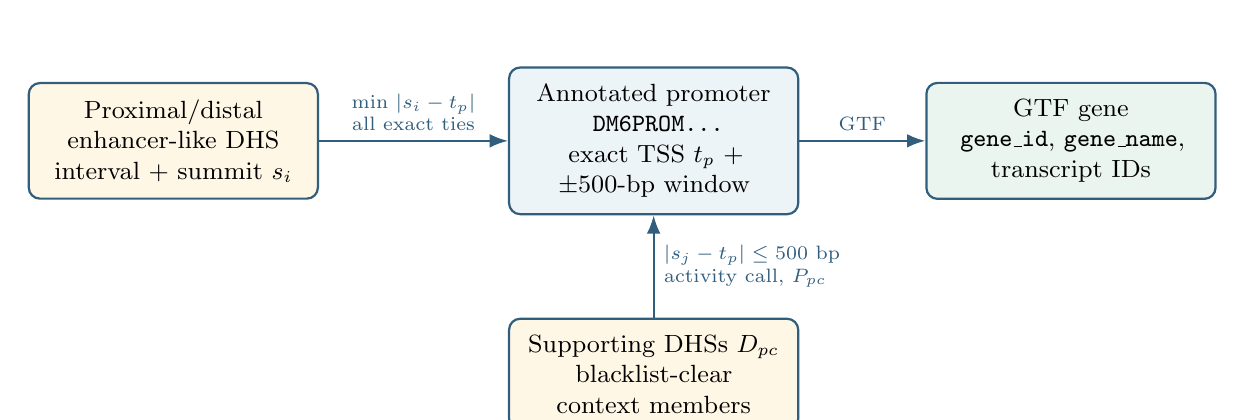
\begin{tikzpicture}[
  >=Latex,
  every node/.style={font=\small,align=center},
  object/.style={draw=pipelineblue,rounded corners,thick,minimum height=1.05cm,
    text width=3.25cm,inner sep=6pt},
  relation/.style={->,thick,color=pipelineblue}
]
  \node[object,fill=lightgold] (enhancer) {Proximal/distal\\enhancer-like DHS\\
    interval + summit $s_i$};
  \node[object,fill=lightblue,right=24mm of enhancer] (promoter) {
    Annotated promoter\\\texttt{DM6PROM\ldots}\\exact TSS $t_p$ + $\pm500$-bp window};
  \node[object,fill=lightgreen,right=16mm of promoter] (gene) {
    GTF gene\\\texttt{gene\_id}, \texttt{gene\_name},\\transcript IDs};
  \node[object,fill=lightgold,below=13mm of promoter] (support) {
    Supporting DHSs $D_{pc}$\\blacklist-clear context members};

  \draw[relation] (enhancer) -- node[above,font=\scriptsize,align=center] {
    min $|s_i-t_p|$\\all exact ties} (promoter);
  \draw[relation] (promoter) -- node[above,font=\scriptsize] {GTF} (gene);
  \draw[relation] (support) -- node[right,font=\scriptsize,align=left] {
    $|s_j-t_p|\leq500$ bp\\activity call, $P_{pc}$} (promoter);
\end{tikzpicture}
\caption{Data types of the nearest-TSS annotation.  Enhancer and supporting DHSs
are master-registry elements whose boundaries are never replaced by the fixed
promoter window.  The nearest promoter is chosen by summit-to-TSS distance
alone; promoter activity in each context is then annotated from blacklist-clear
member DHSs whose summits lie within 500 bp of the TSS.}
\label{fig:nearest-tss}
\end{figure}

\subsection{Starting from a completed catalog}

A completed catalog can be used as the input boundary for a new links-only
result namespace.  \filep{src/create_catalog_manifest.py} writes a one-row TSV
that binds the long catalog, catalog metrics, catalog provenance, and source
resolved configuration by SHA-256.  The manifest also records the source
project, run, method, genome, context order, and semantic digest carried by the
source configuration.

At launch, the pipeline verifies all four files and their internal catalog hash
and requires the supplied accession table to match the sample-sheet hash
recorded by the source catalog.  The link rules stream the long table;
quantification, catalog construction, BigWig generation, and IGV-session
generation are not placed in this DAG.  The original catalog remains immutable
and is referenced only by its manifest and hashes.

\section{Integrated reporting and provenance}

The report endpoint emits deterministic HTML, PDF, and JSON.  Repeated
\texttt{--report-source-root} arguments freeze a bounded set of upstream
manifests, resolved configurations, QC metrics, TSS plots, fragment
histograms, cross-correlation files, MultiQC reports, and master metrics into
the report configuration.  These sources are checked again by SHA-256 during
report construction.

The integrated report summarizes input/output inventories, BAM and FRiP QC,
ATAC TSS and fragment evidence, H3K27ac cross-correlation, master statistics,
TMM factors, regulatory classes, background-percentile activity calls, the
catalog browser assets, and the nearest-TSS enhancer count, tie count, and
per-context number of enhancers whose nearest promoter is active.  Upstream QC
rows are matched to the selected BAMs by checksum.  Its JSON sidecar records
every declared source and current output hash, including BEDs, mean BigWigs,
and IGV sessions.

\subsection{Reproducibility mechanisms}

\begin{itemize}
  \item Rule software is isolated in small pinned Conda environments.
  \item Downloads, reused BAMs, master bundles, report sources, and generated
  exports are checksummed.
  \item Resolved configurations preserve derived defaults and provenance.
  \item Temporary outputs are validated and atomically promoted where
  practical.
  \item Deterministic tables use stable ordering; generated gzip files set a
  fixed modification time; unchanged manifests and provenance files are not
  replaced merely to refresh timestamps.
  \item Snakemake targets express completeness and profiles retain
  \texttt{rerun-incomplete: true}.
  \item A changed scientific semantic digest requires a new \texttt{run\_id}.
\end{itemize}

The run-specific \filep{work/<project>/<run_id>/} tree contains reproducible
intermediates rather than archive products.  Large intermediates---trimmed
FASTQs after alignment, alignment chunks, lane and marked BAMs, shifted or
short-fragment BAMs, peak-calling insertion BEDs, and background-count
tables---are declared temporary and Snakemake removes them after their last
consumer.  Quantification assay-unit BEDs are retained below
\filep{activity/quantification/units/}; they are the strict restart contract
for catalog counting and mean-track construction.  The work directory must
remain available while downstream products are being constructed.  Per-library
H3K27ac CPM BigWigs are not computed because no downstream result consumes
them; pooled ATAC pileup/qpois and context-mean catalog BigWigs are distinct
retained products.  Final replicate-level ATAC peak evidence is archived below
\filep{results/<project>/<run_id>/atac/replicates/} rather than retained under
\filep{work/}.

\section{Principal output inventory}

\begin{longtable}{L{0.24\textwidth} L{0.68\textwidth}}
\toprule
Group & Principal paths below \filep{results/<project>/<run_id>/} \\
\midrule
\endhead
Alignment &
\filep{bam/<library>.final.bam[.bai]};
\filep{qc/alignment/};
\filep{provenance/manifests/final-bams.tsv} \\
QC and review &
\filep{qc/metrics.tsv}, \filep{qc/metrics.json},
\filep{qc/library-review.tsv}, \filep{qc/multiqc/multiqc_report.html},
assay-specific files below \filep{qc/tss/}, \filep{qc/fragments/}, and
\filep{qc/chip/}; H3K27ac QC peaks below \filep{peaks/} \\
Context ATAC &
\filep{atac/conditions/<context>/peaks/} and
\filep{atac/conditions/<context>/tracks/} \\
Master bundle &
\filep{atac/master/master_dhs.bed},
\filep{master_dhs_summits.bed},
\filep{master_dhs_membership.tsv},
\filep{master_dhs_context_matrix.tsv}, and
\filep{master_dhs.json} \\
Quantification &
\filep{activity/quantification/units/*.bed.gz},
\filep{activity/quantification/libraries/*.signal.tsv.gz},
\filep{normalization_factors.tsv}, \filep{context_signal.tsv.gz},
\filep{master_dhs_activity.tsv.gz}, \filep{h3k27ac/master_dhs_signal.tsv.gz},
window counts, metrics, and provenance JSON \\
Catalog &
\filep{activity/catalog/master_elements_long.tsv.gz},
\filep{master_elements_wide.tsv.gz}, \filep{elements/<context>.elements.tsv.gz},
\filep{regulatory_element_summary.tsv},
\filep{regulatory_element_metrics.json}, and
\filep{regulatory_element_provenance.json} \\
Browser bundle &
\filep{activity/catalog/bed/}, \filep{activity/catalog/tracks/},
\filep{activity/catalog/igv/<context>.xml}, and
\filep{activity/catalog/all-contexts.igv.xml} \\
Nearest-TSS links &
\filep{activity/links/nearest_tss/promoters.tsv.gz},
\filep{promoters.metrics.json},
\filep{enhancer_nearest_tss_candidates_wide.tsv.gz}, and its metrics JSON \\
Integrated report &
\filep{activity/report/integrated_qc_report.html},
\filep{integrated_qc_report.pdf}, and
\filep{integrated_qc_report.json} \\
Restart contracts &
\filep{provenance/manifests/<stage>.checkpoint.json} and
\filep{provenance/configs/<stage>.resolved_config.json} at every logical endpoint \\
\bottomrule
\end{longtable}

\section{Reproducing the atlas}

All commands run from the repository root inside the \filep{.venv}
orchestration environment.  The input table is first validated:

\begin{lstlisting}
python src/validate_sample_sheet.py resources/atlas_samples.tsv
\end{lstlisting}

\subsection{Step 1: accessions through QC}

One mixed table produces one QC namespace per assay,
\filep{results/drosophila-atlas.atac.dm6/qc-v1} and
\filep{results/drosophila-atlas.chip_histone.dm6/qc-v1}:

\begin{lstlisting}
python src/run_pipeline.py resources/atlas_samples.tsv \
  --project drosophila-atlas --run-id qc-v1 --genome dm6 \
  --until-stage qc --cores 16
\end{lstlisting}

Adding \texttt{--alignment-chunk-pairs 2000000} enables restartable chunked
alignment of very large lanes.

\subsection{Step 2: apply the QC decisions}

The versioned decision table holds one row per library; \texttt{--assay}
selects the rows for each per-assay manifest:

\begin{lstlisting}
for assay in atac h3k27ac; do
  ns=$([ "$assay" = atac ] && echo atac || echo chip_histone)
  python src/review_final_bam_manifest.py \
    results/drosophila-atlas.$ns.dm6/qc-v1/provenance/manifests/final-bams.tsv \
    --review-table resources/atlas_qc_decisions.tsv --assay "$assay" \
    --output data/reviewed/$assay.reviewed.tsv
done
\end{lstlisting}

\subsection{Step 3: master DHS registry}

The master run reuses the completed QC checkpoint and the reviewed ATAC
manifest; nothing is downloaded or realigned:

\begin{lstlisting}
python src/run_pipeline.py resources/atlas_samples.tsv \
  --from-stage qc \
  --checkpoint-manifest \
    results/drosophila-atlas.atac.dm6/qc-v1/provenance/manifests/qc.checkpoint.json \
  --final-bam-manifest data/reviewed/atac.reviewed.tsv \
  --project drosophila-atlas --run-id master-v1 --genome dm6 \
  --until-stage master --cores 16
\end{lstlisting}

\subsection{Step 4: quantification, catalog, nearest-TSS links, and report}

\begin{lstlisting}
python src/run_pipeline.py resources/atlas_samples.tsv \
  --from-stage master \
  --master-manifest \
    results/drosophila-atlas/master-v1/provenance/manifests/master-dhs.tsv \
  --activity-bam-manifest data/reviewed/atac.reviewed.tsv \
  --activity-bam-manifest data/reviewed/h3k27ac.reviewed.tsv \
  --report-source-root results/drosophila-atlas.atac.dm6/qc-v1 \
  --report-source-root results/drosophila-atlas.chip_histone.dm6/qc-v1 \
  --project drosophila-atlas --run-id catalog-v1 --genome dm6 \
  --until-stage report --cores 16
\end{lstlisting}

The H3K27ac activity threshold defaults to 0.60.  Passing
\texttt{--h3k27ac-activity-threshold T} (\(0<T<1\)) to this command applies
another value; because it changes the scientific result, it requires a new
\texttt{--run-id}.  Adding \texttt{--snakemake-dry-run} to any command shows
the planned jobs, \texttt{--cores} limits total cores, and \texttt{--jobs}
limits concurrent cluster jobs.  Re-running the same command and run ID resumes
valid work.  An earlier endpoint (\stage{quantification}, \stage{catalog}, or
\stage{links}) can be advanced later by passing its exported checkpoint:

\begin{lstlisting}[basicstyle=\ttfamily\footnotesize]
python src/run_pipeline.py resources/atlas_samples.tsv \
  --from-stage quantification \
  --checkpoint-manifest \
    results/drosophila-atlas/catalog-v1/provenance/manifests/quantification.checkpoint.json \
  --until-stage report --cores 16
\end{lstlisting}

\subsection{Links from an exported catalog}

A completed catalog can enter the links stage in a new namespace without
revalidating its BAMs:

\begin{lstlisting}
python src/create_catalog_manifest.py results/drosophila-atlas/catalog-v1 \
  --output data/reviewed/atlas-catalog.tsv
python src/run_pipeline.py resources/atlas_samples.tsv \
  --from-stage catalog --until-stage links \
  --catalog-manifest data/reviewed/atlas-catalog.tsv \
  --project drosophila-atlas --run-id links-v1 --genome dm6
\end{lstlisting}

\section{Default parameters that affect interpretation}

\begin{longtable}{L{0.31\textwidth} L{0.21\textwidth} L{0.39\textwidth}}
\toprule
Parameter & Default & Interpretation \\
\midrule
\endhead
Trim quality / minimum length & 20 / 20 bp & Read-level cleanup before alignment \\
Bowtie2 preset / paired maximum & very-sensitive / 2,000 bp & Alignment sensitivity and allowed concordant span \\
MAPQ / duplicate / mitochondrial filtering & 30 / remove / remove & Final biological-library BAM contract; blacklist alignments are retained \\
ATAC short-fragment maximum & 150 bp, strict & Requires \(0<|\mathrm{TLEN}|<150\) \\
ATAC MACS3 q-value & 0.10 & Lenient candidate stage before geometric refinement \\
qpois exponent range & 2--325 & Progressive signal thresholds \\
qpois retained width & 50--400 bp & Final refined component geometry \\
H3K27ac QC peaks & broad, cutoff 0.1, \(q=0.01\) & IP-only MACS3 call used for QC only \\
Context replicate support & 2 libraries, 0.5 coverage & Minimum reproducibility of pooled peaks \\
Master summit span & 150 bp & Complete-linkage limit across context summits \\
Minimum master summit separation & 50 bp & Close disjoint-context clusters may merge below this distance \\
TMM background bins & 10 kb autosomal & Composition-factor feature space \\
H3K27ac windows & three 500-bp windows & Left, center, and right of the master summit; maximum is used \\
H3K27ac activity threshold \(\tau\) & \(F_c>0.60\), strict & Max3 percentile against blacklist-clear context-nonmember DHSs; \texttt{--h3k27ac-activity-threshold} \\
Blacklist handling & flag; background exclusion & DHSs retained, tested, and flagged; excluded only from \(B_c\) \\
ATAC browser extension & 150 bp & Centered Tn5 insertion pileup recorded in the resolved configuration \\
Promoter/proximal boundaries & 500 / 1,000 bp & Absolute summit-to-nearest-TSS distance \\
Promoter window & 1,000 bp (\(\pm500\)) & Centered on each distinct GTF gene/TSS \\
Promoter activity support & inclusive 500 bp & Blacklist-clear catalog-active member DHS summit within 500 bp of the TSS \\
Nearest-TSS enhancer activity & no filter & Every proximal/distal enhancer receives one row; activity is a context annotation \\
Nearest-TSS distance & no cutoff & Minimum same-chromosome summit-to-TSS distance; exact ties retained in one row \\
\bottomrule
\end{longtable}

\section{Pinned principal software}

The rule environments pin the principal tools shown below; the orchestration
environment pins Snakemake.  The resolved Conda environments and report
receipts remain the authoritative record for an individual run.

\begin{center}
\begin{tabular}{ll@{\qquad}ll}
\toprule
Tool & Version & Tool & Version \\
\midrule
Snakemake & 9.23.1 & Bowtie2 & 2.5.5 \\
samtools & 1.23.1 & bedtools & 2.31.1 \\
FastQC & 0.12.1 & Cutadapt & 5.2 \\
MACS3 & 3.0.4 & deepTools & 3.5.6 \\
MultiQC & 1.35 & phantompeakqualtools & 1.2.2 \\
R & 4.5.3 & edgeR & 4.8.2 \\
pyBigWig & 0.3.25 & WeasyPrint & 66.0 \\
aria2 & 1.37.0 & Python & 3.11 \\
\bottomrule
\end{tabular}
\end{center}

\section{Interpretive cautions}

\begin{itemize}
  \item A refined qpois component inherits its candidate call; refinement is
  not a new independent false-discovery-rate procedure.
  \item Replicate support is interval coverage of a pooled peak, not a test of
  identical peak boundaries or identical signal magnitude.
  \item A master DHS represents compatible accessibility evidence across
  contexts.  It is not a fixed-width enhancer, a gene assignment, or a claim
  that the element is active in every context.
  \item H3K27ac QC peaks are called without an input control.  They inform
  library review only and do not enter the catalog.
  \item Background TMM assumes that a useful reference composition can be
  estimated from autosomal bins.  Factor ranges, library QC, and signal
  distributions should be inspected for strong global or technical shifts.
  \item The empirical max3 background percentile is a relative,
  context-specific activity measure.  Its value depends on the
  context-nonmember background and the chosen threshold, and it is not a
  calibrated probability of enhancer function.
  \item A blacklist overlap is a technical warning, not proof that an element
  is artifactual.  Conversely, retaining the reads can allow blacklist-driven
  signal to affect peak calling and activity calls, so analyses should state
  whether they filter on \texttt{blacklist\_overlap}.
  \item TSS-proximity classes are annotation categories.  Distal or proximal
  labels do not establish enhancer function, and the nearest annotated TSS is
  a proximity baseline, not a demonstrated regulatory target.
  \item Browser tracks are normalized context means intended for inspection;
  replicate-level tables and standard deviations remain necessary for
  uncertainty assessment.
\end{itemize}

\section{Verification of this description}

This document was written against the current sample-sheet schema, launcher,
configuration validators, \filep{workflow/Snakefile}, all included rule files,
the master/consensus/activity/catalog/nearest-TSS implementations, the README,
and the workflow environment files.  To rebuild the PDF from the repository
root with auxiliary files kept outside the repository:

\begin{lstlisting}
latexmk -pdf -interaction=nonstopmode -halt-on-error \
  -output-directory="$(mktemp -d)" docs/pipeline-description.tex
\end{lstlisting}

and copy the resulting PDF to \filep{docs/pipeline-description.pdf}.

For a scientific run, documentation review is not sufficient verification.
Validate the sample sheet, inspect the resolved configuration and semantic
digest, run an appropriate Snakemake dry-run, review library QC decisions, and
retain the generated manifests and report JSON with the results.

\end{document}
